\documentclass[11pt,letterpaper]{article}
\usepackage[top=0.85in,left=2.00in,footskip=0.75in]{geometry}
\usepackage[titletoc,page]{appendix}
% Use adjustwidth environment to exceed column width (see example table in text)
\usepackage{changepage}
\usepackage[english]{babel}
\usepackage{booktabs}
\usepackage{siunitx}%Questo serve a caricare il pacchetto delle unità di misura del sistema internazionale%
\usepackage[utf8]{inputenc}
\usepackage{graphicx} 
\usepackage{url}
\usepackage{amsmath}
\usepackage{amssymb}
\usepackage{listings}


\usepackage{keyval}
\usepackage{xcolor}
\usepackage{caption}
\usepackage{tikz}
\usepackage{circuitikz}
\usepackage{authblk}
%\usepackage{hyperref}


\usepackage[lofdepth,lotdepth]{subfig}
% Remove comment for double spacing
%\usepackage{setspace} 
%\doublespacing
% Text layout
%\raggedright
\setlength{\parindent}{0.5cm}
\textwidth 5.25in 
\textheight 8.75in

\usepackage[aboveskip=1pt,labelfont=bf,labelsep=period,justification=raggedright,singlelinecheck=off]{caption}

% Use the PLoS provided BiBTeX style
\bibliographystyle{plos2009}

% Remove brackets from numbering in List of References
\makeatletter
\renewcommand{\@biblabel}[1]{\quad#1.}
\makeatother


\begin{document}
\vspace*{0.30in}

\begin{flushleft}
{\Large
\textbf\newline{\textbf{Black Scholes Formula}}
}
\newline
% Insert Author names, affiliations and corresponding author email.
\\
Lorenzo Maria Perrone\textsuperscript{1, *}
%Name2 Surname\textsuperscript{2,\textpilcrow},
%Name3 Surname\textsuperscript{2,\textcurrency a},
%Name4 Surname\textsuperscript{2,\ddag},
%Name5 Surname\textsuperscript{2,\ddag},
%Name6 Surname\textsuperscript{2,\Yinyang},
%Name7 Surname\textsuperscript{3,*,\Yinyang}
\\
\bf{1} Department of Physics, EPFL
\\
%\bf{2} Affiliation Dept/Program/Center, Institution Name, City, State, Country
%\\
%\bf{3} Affiliation Dept/Program/Center, Institution Name, City, State, Country
%\\

% Insert additional author notes using the symbols described below. Insert symbol callouts after author names as necessary.
% 
% Remove or comment out the author notes below if they aren't used.
%
% Primary Equal Contribution Note
%\Yinyang These authors contributed equally to this work.

% Additional Equal Contribution Note
%\ddag These authors also contributed equally to this work.

% Current address notes
%\textcurrency a Insert current address of first author with an address update
% \textcurrency b Insert current address of second author with an address update
% \textcurrency c Insert current address of third author with an address update

% Deceased author note
%\dag Deceased

% Group/Consortium Author Note
%\textpilcrow Insert Collaborative Author line here

* E-mail: lorenzo.perrone@epfl.ch
\end{flushleft}

\begin{lstlisting}

# -*- coding: utf-8 -*-
"""
Created on Wed Mar 15 15:16:20 2017

@author: LorenzoLMP
"""
from pylab import *  
from scipy import * 
from scipy.stats import norm

def d1(x, c, s, r, tau, t):
    return (log(x/c) + (r + 0.5*s**2)*(tau-t))/(s*sqrt(tau-t))

def d2(x, c, s, r, tau, t):
    return (log(x/c) + (r - 0.5*s**2)*(tau-t))/(s*sqrt(tau-t))
    
def w(x, c, r, t, tau, d1, d2):
    return x*norm.cdf(d1) - c*exp(r*(t-tau))*norm.cdf(d2)

#DEFINITION OF PARAMETERS
c = 20
s = sqrt(0.2)
r = 1
tau = 1
t1 = 0.1
t2 = 0.5
t3 = 0.8
t4 = 0.99
    
rc('font', size=14)
xlabel(r' $X(t)$ [$ \$ $]')
ylabel(r'Option price $w(X,t)$ [$ \$ $]')
minorticks_on()
grid(which='major')
#yscale('log')
#xscale('log')
title("Option Price vs Stock Price")
xdata = linspace(0.1, 40, 30)
xxdata = linspace(0.1, 40, 200)
xxxdata = linspace(20, 40, 100)
plot(xdata, w(xdata, c, r, t1, tau, d1(xdata, c, s, r, tau, t1), d2(xdata, c, s, r, tau, t1)), linestyle='None', marker= 'o', color="red", label='t1=0.1')
plot(xdata, w(xdata, c, r, t2, tau, d1(xdata, c, s, r, tau, t2), d2(xdata, c, s, r, tau, t2)), linestyle='None', marker= '^', color="b",label='t2=0.5')
plot(xdata, w(xdata, c, r, t4, tau, d1(xdata, c, s, r, tau, t4), d2(xdata, c, s, r, tau, t4)), linestyle='None', marker= 'd', color="orange", label='t3=0.8')
plot(xdata, w(xdata, c, r, t3, tau, d1(xdata, c, s, r, tau, t3), d2(xdata, c, s, r, tau, t3)), linestyle='None', marker= 's', color="g",label='t4=0.99')
plot(xxdata, xxdata, linestyle='-',color="k", label='max. option')
plot(xxxdata, xxxdata-c, linestyle='--',color="k", label='min. option')
legend(loc='upper left')
savefig('black_scholes.png', dpi=600)
show()

\end{lstlisting}

\begin{figure}
\centering
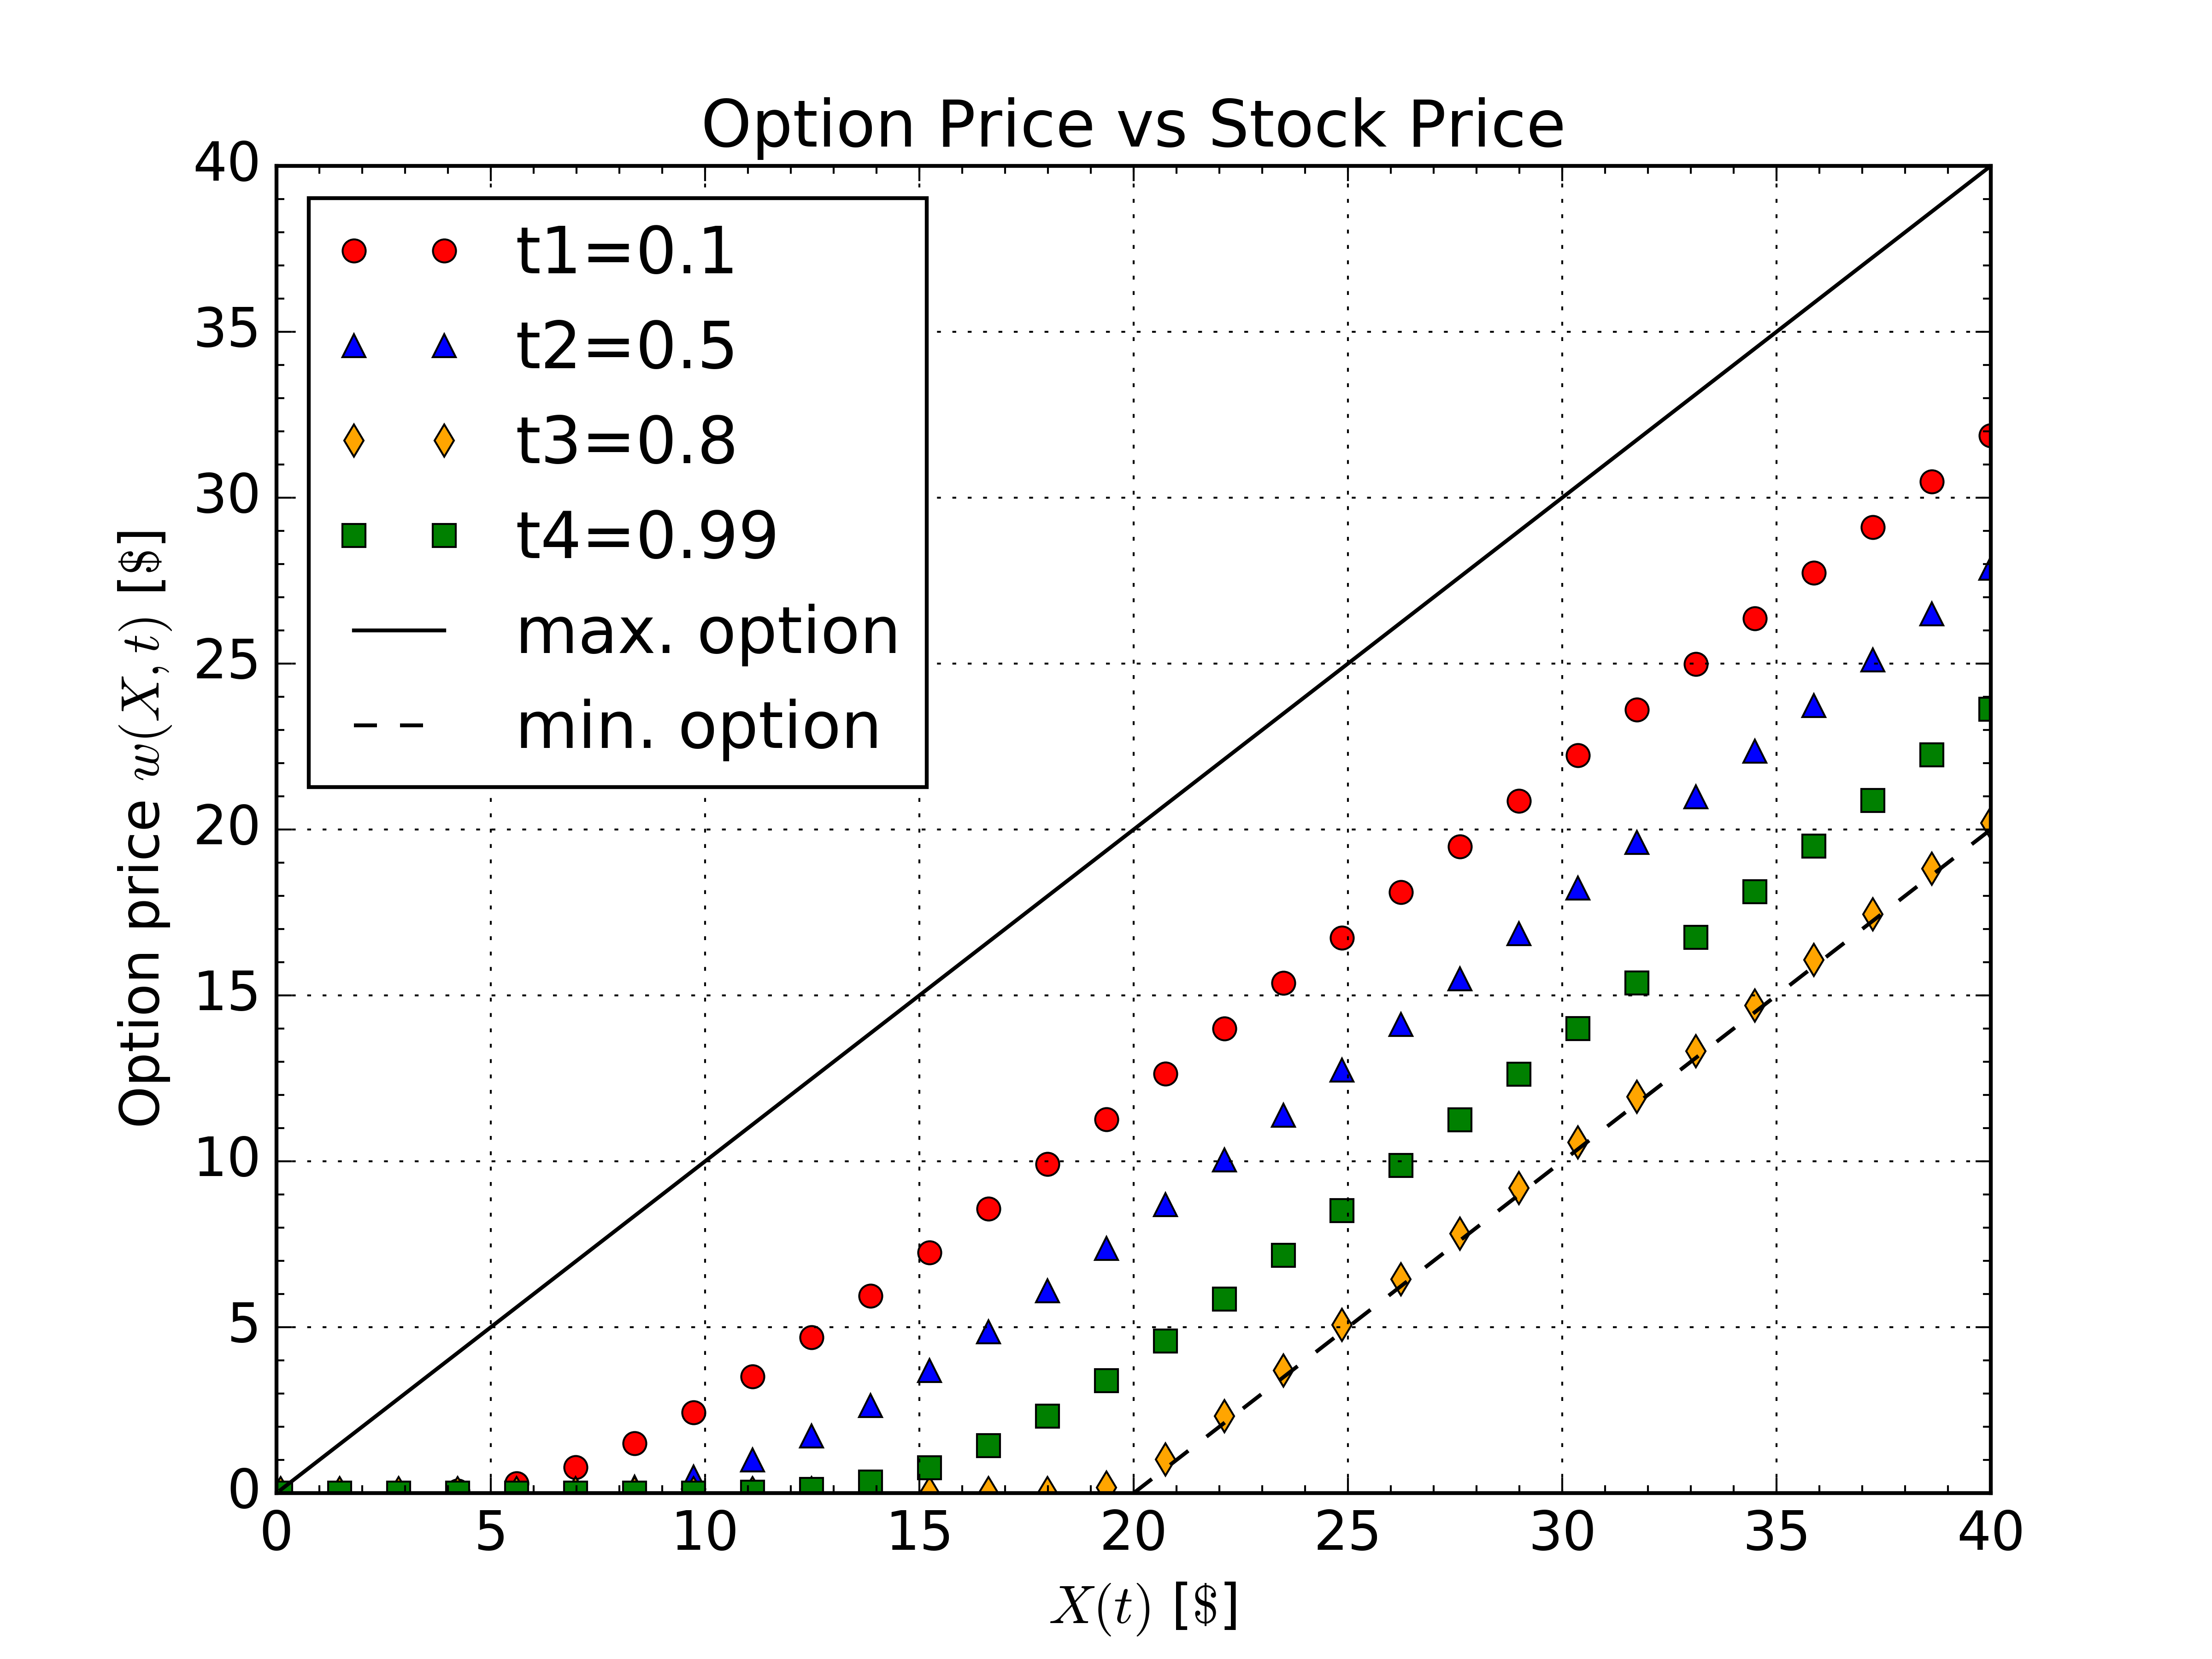
\includegraphics[width=0.9\linewidth]{./black_scholes}
\caption{Option price as a function of stock price for different times. Maturity $ t^*$ set to 1.}
\label{fig:black_scholes}
\end{figure}


\end{document}